% Template for ICIP-2009 paper; to be used with:
%          spconf.sty  - ICASSP/ICIP LaTeX style file, and
%          IEEEbib.bst - IEEE bibliography style file.
% --------------------------------------------------------------------------
\documentclass{article}
\usepackage{spconf,amsmath,epsfig,subfig,graphicx,algorithm,algorithmic,subfig,multirow}

% Example definitions.
% --------------------
\def\x{{\mathbf x}}
\def\L{{\cal L}}

% Title.
% ------
\title{ROBUST LANE DETECTION AND TRACKING WITH RANSAC AND KALMAN FILTER}
%
% Single address.
% ---------------
%\name{Amol Borkar, Monson H. Hayes, Mark T. Smith}
%\address{Address}
%\name{\begin{tabular}[t]{c@{\extracolsep{8em}}c}
%I. M. Anonymous  & M. Y. Coauthor\\
% \\
%        My Department & Coauthor Department\\
%        My Institute & Coauthor Institute\\
%        City, STATE~~zipcode & City, STATE~~zipcode
%\end{tabular}}
%\address{}

% For example:
% ------------
%\address{School\\
%	Department\\
%	Address}
%
% Two addresses (uncomment and modify for two-address case).
% ----------------------------------------------------------
\twoauthors
  {Amol Borkar, Monson Hayes}
	{\small{Center for Signal and Image Processing (CSIP)}\\
	\small{Georgia Institute of Technology}\\
	\small{Atlanta, GA}\\
    \small{$\{$amol,mhh3$\}$@gatech.edu}}
  {Mark T. Smith}
	{\small{Institut f\"{o}r Till\"{a}mpad Informationsteknik}\\
    \small{Kungliga Tekniska H\"{o}gskolan}\\
	\small{Stockholm, Sweden}\\
    \small{msmith@kth.se}}
%
\begin{document}
%\ninept
%
\maketitle
%
\begin{abstract}
In a previous paper, a simple approach to lane detection using the Hough
transform and iterated matched filters was described \cite{borkar_layered_2009}.
This paper extends this work by incorporating an inverse perspective mapping
to create a bird's-eye view of the road, applying random sample consensus to help
eliminate outliers due to noise and artifacts in the road, and a Kalman filter
to help smooth the output of the lane tracker.
\end{abstract}
%
\begin{keywords}
Lane detection, Hough transform, Kalman filter.
\end{keywords}
%
\section{Introduction}
\label{sec:intro}
Driver safety on the highways has been an area of interest for many years.
With the development of fast, cheap, low-power, and sophisticated electronics,
automobiles with sensors, electronics, and warning systems are beginning to appear on the market.

One of the interesting areas of research and development is collision avoidance.
An important component for effective collision avoidance is lane detection.
The ability to detect sudden or unexpected lane changes when there
is traffic in the lane a driver is moving into could help a driver to avoid
collisions.
Effective monitoring of the position of a car within a lane could be used to
help avert a collision due to driver distractions, fatigue, or driving under the influence of a controlled substance.
There are obvious difficulties and challenges in designing collision avoidance
systems, and some of the challenges fall outside the realm of engineering and
involve complicated issues related to law and liability.

In this paper, we address some of the image processing challenges is designing a
lane detection system.  It is organized as follows.
After a brief survey of some previous research, we then describe the various
components of the system.  These include image pre-processing using temporal blurring,
inverse projective mapping to create a bird's-eye view of the road, a Hough transform
for detecting candidate lane markers, a random sample consensus algorithm to
help deal with outliers in the image, and tracking of the lane parameters using a Kalman filter.
Then, we briefly describe the hardware that was used to collect data, and
then show the performance of the lane tracking system.
It is shown that this system exhibits considerable improvement in
performance compared to a system using only the Hough transform and matched filtering that was previously described \cite{borkar_layered_2009}.

\section{Prior Research}
\label{sec:prior}
Numerous techniques for vision-based lane detection have been developed in an attempt to robustly detect lanes.
In the extraction of features for lane detection, one of the most commonly used approaches it to apply an edge detector to the data \cite{assidiq_real_2008,wang_driver_2005}. With this approach, a Canny edge detector is typically used to generate a binary edge map. From the binary edge map, the classical Hough transform is then used to extract a set of lines as candidates for the lane markers.  While this approach shows good results in general, the detected lanes are often skewed due to surface irregularities or navigational text markers on the road. Color segmentation to extract lane markers is another approach that is often used \cite{sun_hsi_2006,chin_lane_2005}. Unfortunately, color segmentation is sensitive to ambient light and requires additional processing to avoid undesirable effects.

The majority of the approaches used for lane detection operate directly on the images that are captured by the camera without any geometrical correction or change in camera perspective \cite{borkar_layered_2009,assidiq_real_2008,sun_hsi_2006,wang_real-time_2006}.
Although dealing with images from the camera perspective allows access to raw data values, defining the properties of the features of interest may be complicated. For example, a forward-looking camera will capture images that have lane markers that are not parallel and have line widths that vary as a function of the distance from the camera.  These variations often necessitate processing each row of a captured image in a different manner.

Many of the systems described above perform well under certain driving conditions and often require that a certain set assumptions are valid.  Some of these assumptions include the  presence of strong lane marker contrast and roads devoid of artifacts such as cracks, arrows, or similar markers. Unfortunately, these assumptions do not hold in many high traffic urban streets and highways.

\section{Methodology}
\label{sec:methodology}
This paper extends the layered lane detection approach in \cite{borkar_layered_2009} by (1) using an inverse perspective mapping, (2) applying a random sample consensus to help eliminate outliers, and (3) using a Kalman filter for prediction and smoothing.
In the following sections, the various components of the lane detection system are described.
\subsection{Image Enhancement}
The captured color images undergo a grayscale transformation and temporal blurring by averaging $N=3$ successive frames.  This smoothing helps connect dashed lane markers to form a near continuous line \cite{borkar_layered_2009}.
\subsection{Inverse Perspective Mapping}
The next step is to perform an inverse perspective mapping (IPM) on the images.  This transformation is used to change the captured images from a camera perspective to a bird's-eye view as illustrated in Fig. \ref{fig:ipm}.
\cite{sehestedt_robust_2007,shu_vision_2004,bertozzi_gold:parallel_1998}.
\begin{figure}[htb]
  \centering
    \subfloat[Camera perspective view.]{\label{fig:cam_pers}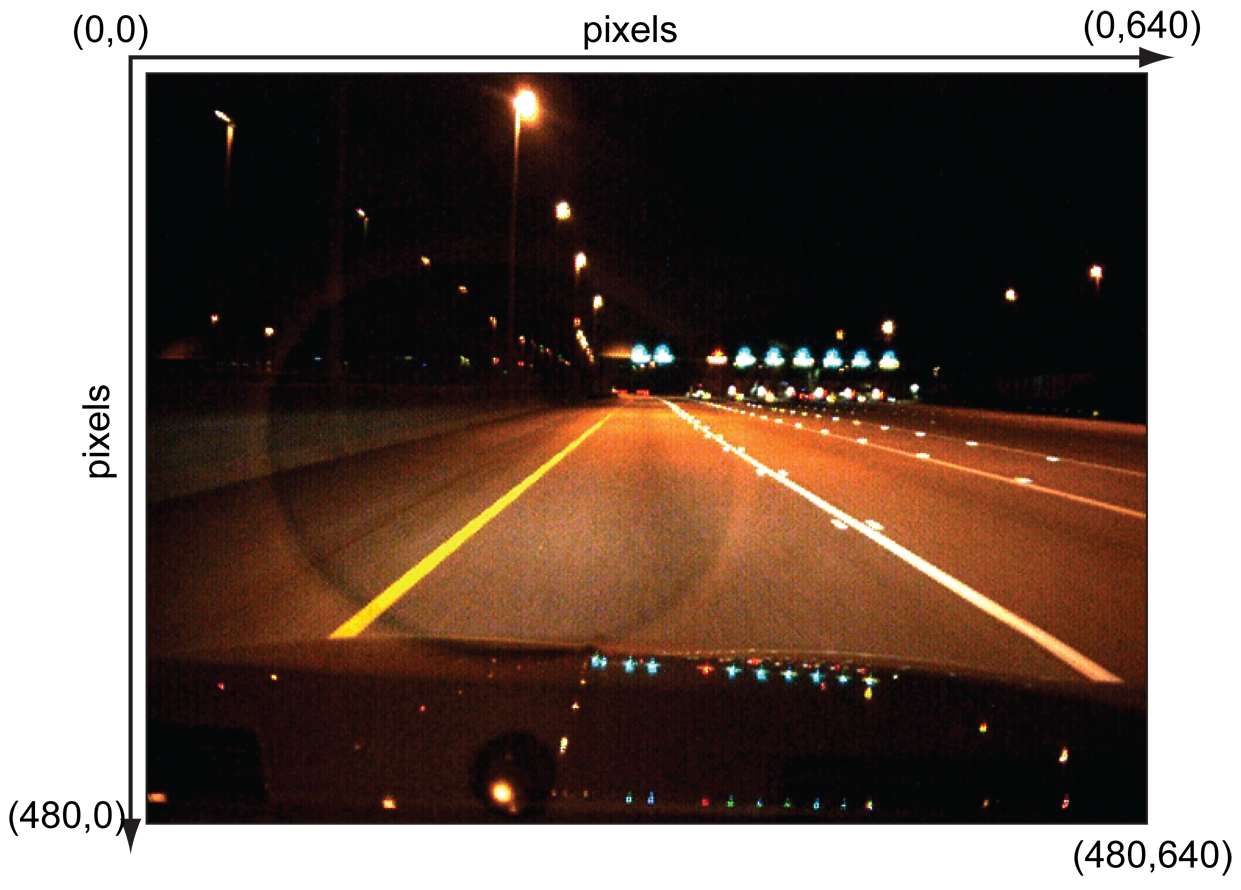
\includegraphics[width=0.235\textwidth]{IMG/ipm11.png}}\hspace{0.00001in}
      \subfloat[Bird's-eye view.]{\label{fig:ipm_feet}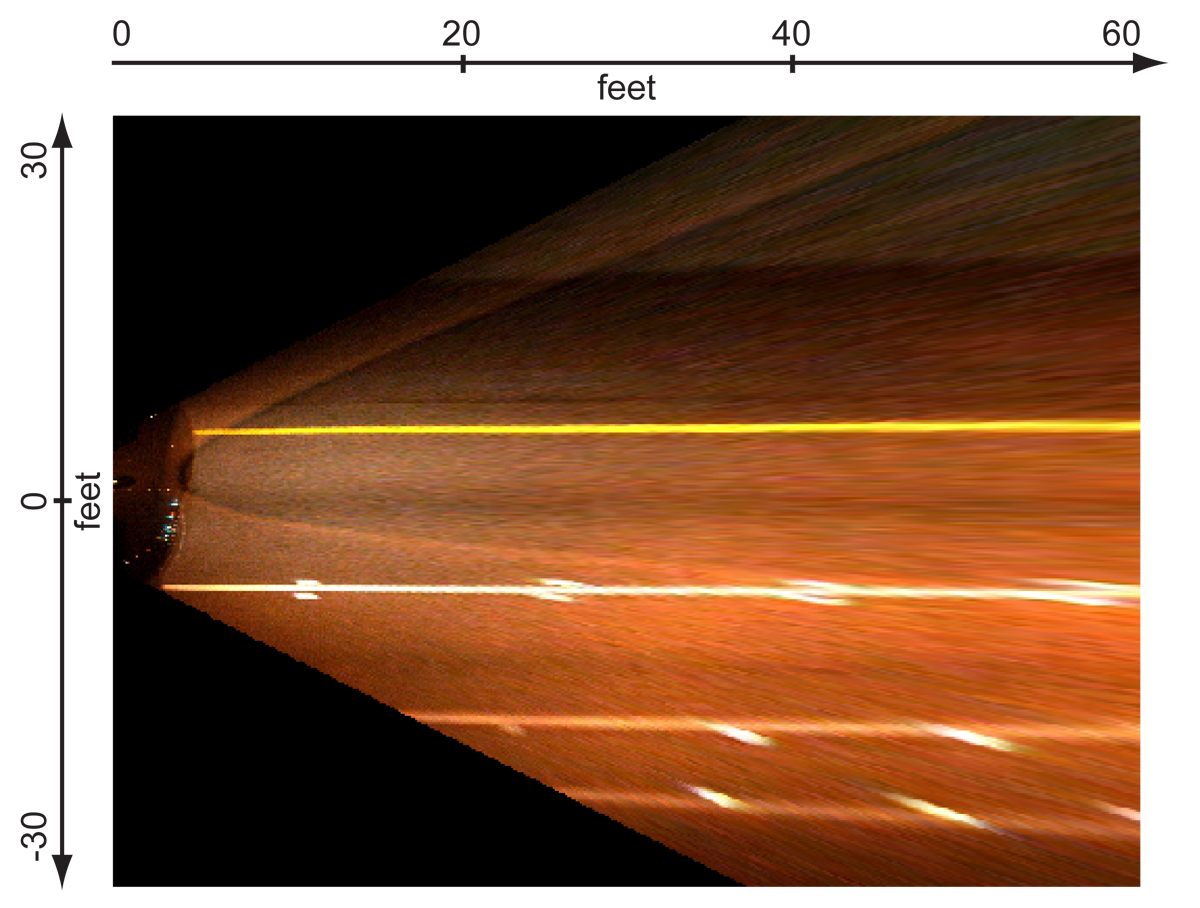
\includegraphics[width=0.235\textwidth]{IMG/ipm22.png}}\\
    %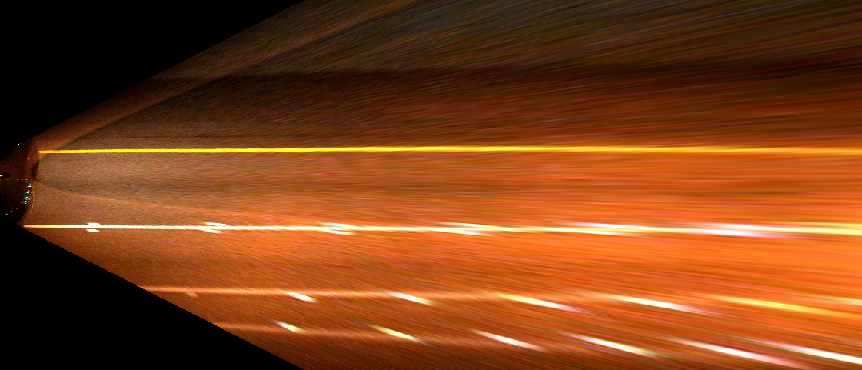
\includegraphics[width=0.45\textwidth]{IMG/ipm_fwd.png}
  \caption{Inverse perspective mapping transforms a camera perspective image into a bird's-eye view image.}
  \label{fig:ipm}
\end{figure}
With this transformation, lane detection now becomes a problem of detecting a pair of parallel lines that are generally separated by a given, fixed distance.
%The benefit of this approach is the simplification of lane marker detection and %classification as the initially converging lane marker sequences now appear parallel.
In addition, this transformation enables a mapping between pixels in the image plane to world co-ordinates (feet) as shown in Fig. \ref{fig:ipm_feet}. The camera's intrinsic and extrinsic parameters are necessary to ensure an accurate transformation.
\subsection{Lane Candidate Location Detection}
Next, an adaptive threshold is applied to the IPM image to generate a binary image \cite{borkar_layered_2009}. Each binary image is then split into two two halves, each one presumably containing one lane marker.
A low-resolution Hough transform is then computed on the binary images and the ten highest scoring lines are found for each half image \cite{borkar_layered_2009}. Each line is then sampled along its length at a specified distance as illustrated by the red plus signs in Fig. \ref{fig:sampling_points}.
%This is further illustrated in Fig. \ref{fig:sampling_points}, where the red lines symbolize the lines detected by computing the Hough transform, and, the yellow lines symbolize the discrete sampling locations.
%The corresponding location of each of these points in the IPM average image is recovered.
\begin{figure}[htb]
  \centering
  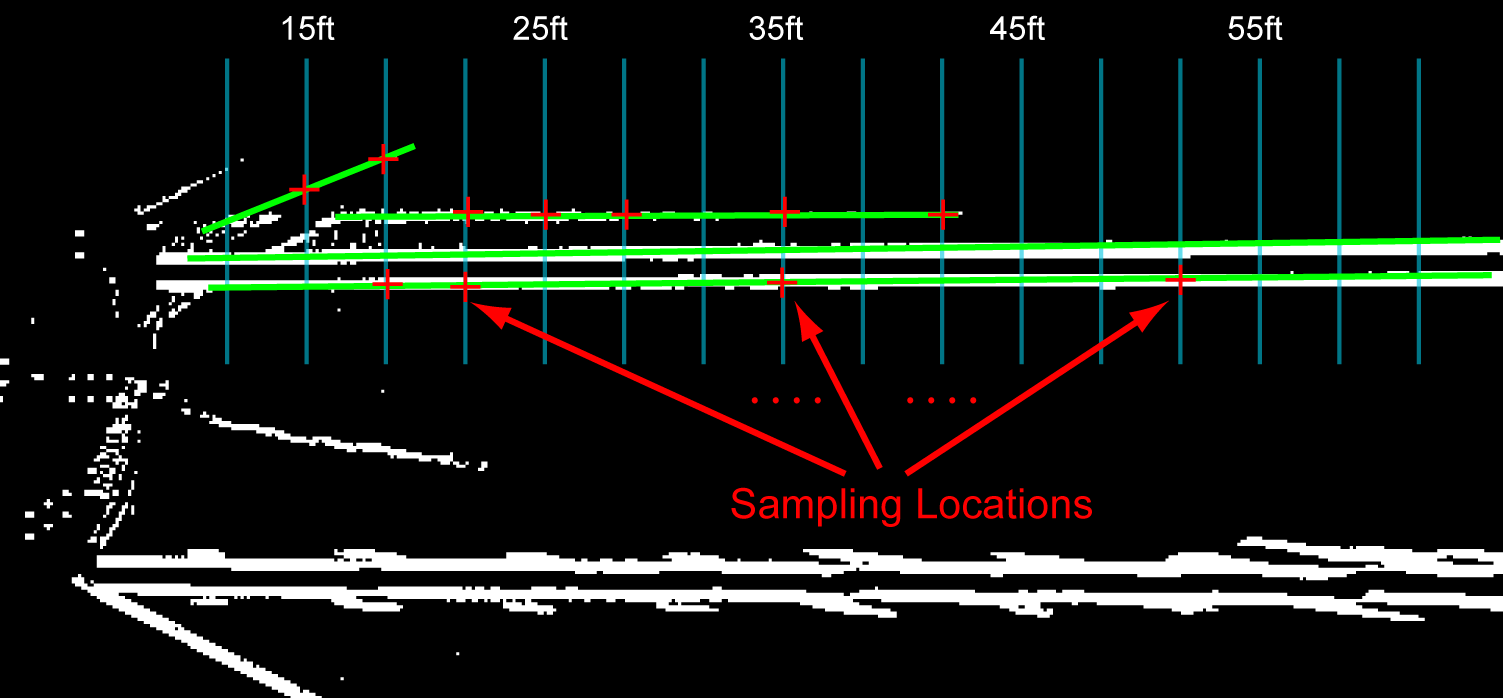
\includegraphics[width=0.45\textwidth]{IMG/cand_lane_points.png}
  \caption{The green lines represent high-scoring lines from the Hough transform, and the plus signs indicate the points where each line is to be sampled.}
  \label{fig:sampling_points}
\end{figure}
To find the approximate center of each line, a one-dimensional matched filter is applied at each sample point along each line.
As described in \cite{borkar_layered_2009}, the matched filter is a Gaussian with a variance that is a function of the line width.
Since the bird's-eye view created with the IPM produces lines of approximately constant width, a fixed variance Gaussian kernel may be used for the matched filter.
%This was not the case in \cite{borkar_layered_2009} where a variety of variances had to be used to create the kernel on different scanlines. Matched filtering is iteratively performed on the remaining X-1 lines.
%As each of the X lines is sampled at the specific co-ordinates, X filtering results are available at each of these positions upon completing the iterations.
After the matched filtering, the pixel with the largest correlation coefficient at each sample point is selected as the best estimate of the center of the lane marker as indicated by the green plus signs in Fig. \ref{fig:cand_pts}.
\begin{figure}[htb]
  \centering
  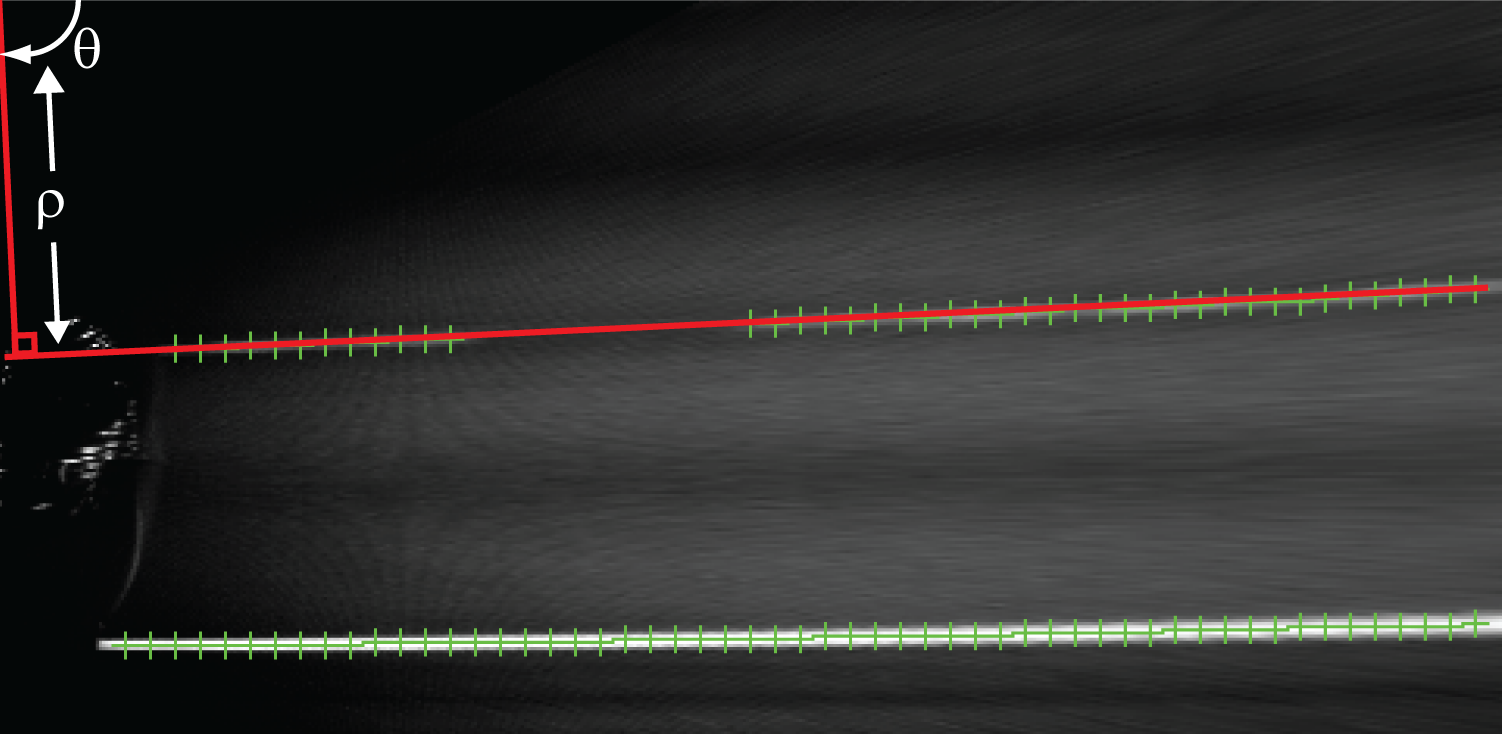
\includegraphics[width=0.45\textwidth]{IMG/rho_theta.png}
  \caption{Line fitted through one set of candidate points and parameterized with $\rho$ and $\theta$.}
  \label{fig:cand_pts}
\end{figure}
\subsection{Outlier Elimination and Data Modeling}
Once the center of each candidate line at each sample point has been estimated, Random Sample Consensus (RANSAC) is applied to the data points. The generic RANSAC algorithm robustly fits a model through the most probable data set or inliers while rejecting outliers \cite{hartley_multiple_2004,fischler_random_1981}. Linear Least Squares Estimation (LSE) is then used to fit to a line on the inliers. Fig. \ref{fig:cand_pts} illustrates the parametrization of the fitted line in terms of $\rho$ and $\theta$ where $\rho$ is the distance from the origin (top left corner pixel) to the line and $\theta$ is the angle as indicated in Fig. \ref{fig:cand_pts} (generally is close to $90^\circ$).
%The orientation of line is specified by $\rho$ (vertical distance to the line from the origin, which is the top left corner pixel) and $\theta$ (the angle of the line, which generally is close to zero degrees).
%For data fitting, a line was chosen over a parabolic fit since the latter is more sensitive to minor perturbations within the inliers, this can result sometimes in desirably shaped curves.\\
\subsection{Tracking}
The parameters of each line is predicted using a Kalman filter.
The state vector \textbf{x}($n$) and observation vector \textbf{y}($n$) are defined as
\begin{equation}
    {\bf x}(n)= {\bf y}(n)
     = \left[ \begin{array}{cccc}
        \rho (n) & \dot{\rho}(n) & \theta (n) & \dot{\theta}(n)
        \end{array} \right]^T
\label{eq:state_measure_vectors}
\end{equation}\\
where $\rho$ and $\theta$ define the line orientation and $\dot{\rho}$ and $\dot{\theta}$ are the derivatives of $\rho$ and $\theta$ that are estimated using the difference in $\rho $ and $\theta $ between the current and previous frame.
The state transition matrix $A$ is
%and observation model $C$ are defined as
\begin{equation}
A = \begin{bmatrix} 1 && 1 && 0 && 0 \\ 0 && 1 && 0 && 0 \\ 0 && 0 && 1 && 1 \\ 0 && 0 && 0 && 1 \\\end{bmatrix}\\
\label{eq:state_trans}
\end{equation}\\
and the matrix $C$ in the measurement equation is the identity matrix.
%\begin{equation}
%C = \begin{bmatrix} 1 && 0 && 0 && 0 \\ 0 && 1 && 0 && 0 \\ 0 && 0 && 1 && 0 \\ 0 && 0 && %0 && 1 \\\end{bmatrix}\\
%\label{eq:observation_model}
%\end{equation}\\
%Independence between parameters $\rho$, $\theta$, $\dot{\rho}$ and $\dot{\theta}$ allows creation of simple covariance matrices $Q_w$ and $Q_v$. $Q_w$ and $Q_v$ represent the process and observation noise respectively \cite{hayes_statistical_1996}.
%\begin{algorithm}[htb]
%\caption{Kalman filter implementation}
%\label{algo:Kalman_Implementation}
%\begin{algorithmic}[1]
%\FOR{($n$=Current Frame)}
%\STATE $\hat{x}(n|n-1)=A(n-1)\hat{x}(n-1|n-1)$
%\STATE $P(n|n-1)=A(n-1)P(n-1|n-1)A^H(n-1)+Q_w(n)$
%\STATE $K(n)=P(n-1|n-1)C^H(n)[C(n)P(n|n-1)C^H(n)+Q_v(n)]^{-1}$
%\STATE $\hat{x}(n|n)=\hat{x}(n|n-1)+K(n)[y(n)-C(n)\hat{x}(n|n-1)]$
%\STATE $P(n|n)=[I-K(n)C(n)]P(n|n-1)$
%\ENDFOR
%\end{algorithmic}
%\end{algorithm}
The noise in the state and measurement equations is assumed to be white
and each process is assumed to be uncorrelated with the others.
Therefore, the covariance matrices for these vector random processes are
constant and diagonal. The variance of each noise process is estimated
 off-line using frames in which accurate estimates
of the lanes were being produced.
The Kalman filter recursively predicts the parameters in the state vector from the previously available information \cite{hayes_statistical_1996,brookner_tracking_1998}.
%$P(n)$ and $K(n)$ represent error covariance matrix and optimal Kalman gain.
In the case of a lane markers not being detected, the matrix $C$ is set to zero
%the values in $Q_v$ are increased significantly and $\hat{x}(n|n)$ is modified as follows
%\begin{equation}
%\hat{x}(n|n) = \hat{x}(n|n-1)
%\label{eq:xnn_mod}
%\end{equation}\\
forcing the Kalman filter to rely purely on prediction.

Finally, the estimated line is mapped back to the camera perspective to portray the lane detection results.

\section{Experimental Analysis}
\label{sec:exp_ana}
\subsection{Hardware}
The hardware used to test and evaluate this new lane detection system is built around an Intel based computer.  A forward facing Firewire color camera is installed below the rear-view mirror so that it has a clear view of the road ahead. The Firewire allows video to be captured at VGA resolution and 30fps.
Video from the camera is recorded onto hard disks.
\subsection{Results}
The lane detection algorithm was implemented in Matlab and requires
approximately 0.8 seconds to process each frame.
Table \ref{tab:laneDetectionCompare} and Table \ref{tab:laneDetectionCompare2} illustrate the performance of the current and previous lane detection systems when applied to over 10 hours of captured video. The results in Table \ref{tab:laneDetectionCompare} show an improvement in accuracy over the system described in \cite{borkar_layered_2009}. The lack of accessibility to other lane detection algorithms and turnkey software systems makes it extremely difficult to compare results.
%\begin{table}[htb!]
%\caption{Accuracy of the lane detection system}
%\label{tab:laneDetectionCompare}
%\resizebox{0.48\textwidth}{!}{
%\begin{tabular}{|p{0.065\textwidth}|p{0.055\textwidth}|p{0.065\textwidth}|p{0.065\textwidth}|p{0.065\textwidth}|p{0.065\textwidth}|p{0.065\textwidth}|p{0.065\textwidth}|}
%\hline
%& & \multicolumn{6}{|c|}{Average Detection Rate Per Minute} \\ \cline{3-8}
%\multirow{2}{*}{Road} & \multirow{2}{*}{Traffic} & \multicolumn{3}{|c|}{Current System} & \multicolumn{3}{|c|}{Previous System \cite{borkar_layered_2009}}\\ \cline{3-8}
%& & Correct & Incorrect & Misses & Correct & Incorrect & Missed\\ \hline
%%\multirow{2}{*}{Isolated} & Light & 99.08\% & 0.99\% & 0\% & 89.69\% & 5.31\% & 5.19\%\\ \cline{2-8}
%Isolated & Light & 99.08\% & 0.99\% & 0\% & 89.69\% & 5.31\% & 5.19\%\\ \cline{2-8}
%Highway & Mod. & 98.34\% & \normalsize{1.65\%} & 0\% & 91.47\% & 6.65\% & 1.87\%\\ \hline
%Metro & Light & 98.37\% & 1.65\% & 0\% & 83.53\% & 8.89\% & 8.14\%\\ \cline{2-8}
%Highway & Mod. & 96.34\% & 3.65\% & 0\% & 84.97\% & 10.33\% & 4.68\%\\ \hline
%\multirow{1}{*}{City} & Variable & 86.39\% & 12.71\% & 0.78\% & 76.55\% & 11.94\% & 11.95\%\\ \hline
%\end{tabular}}
%\end{table}\\
The captured videos contain scenes with a variety of traffic and illumination conditions that depict environments a driver might encounter \cite{borkar_layered_2009}. Fig. \ref{fig:lane_detection} shows a few of instances of detected lane markers.
The results are quantified in terms of detection rate per minute. This metric allows to normalize the results when data is captured using cameras with different frame rates.
\begin{table}[htb!]
\caption{Accuracy of the current lane detection system}
\label{tab:laneDetectionCompare}
\resizebox{0.48\textwidth}{!}{
\begin{tabular}{|p{0.08\textwidth}|p{0.07\textwidth}|p{0.065\textwidth}|p{0.065\textwidth}|p{0.065\textwidth}|}
\hline
%& & \multicolumn{3}{|c|}{Avg. Detection Rate Per Minute} \\ \cline{3-5}
\multirow{2}{*}{Road Type} & \multirow{2}{*}{Traffic} & \multicolumn{3}{|c|}{Avg. Detection Rate Per Minute} \\ \cline{3-5}
& & Correct & Incorrect & Misses \\ \hline
%\multirow{2}{*}{Isolated} & Light & 99.08\% & 0.99\% & 0\% & 89.69\% & 5.31\% & 5.19\%\\ \cline{2-8}
Isolated & Light & 99.08\% & 0.99\% & 0\% \\ \cline{2-5}
Highway & Moderate & 98.34\% & 1.65\% & 0\% \\ \hline
Metro & Light & 98.37\% & 1.65\% & 0\% \\ \cline{2-5}
Highway & Moderate & 96.34\% & 3.65\% & 0\% \\ \hline
\multirow{1}{*}{City} & Variable & 86.39\% & 12.71\% & 0.78\% \\ \hline
\end{tabular}}
\end{table}\\
\begin{table}[htb!]
\caption{Accuracy of the previous lane detection system \cite{borkar_layered_2009}}
\label{tab:laneDetectionCompare2}
\resizebox{0.48\textwidth}{!}{
\begin{tabular}{|p{0.08\textwidth}|p{0.07\textwidth}|p{0.065\textwidth}|p{0.065\textwidth}|p{0.065\textwidth}|}
\hline
%& & \multicolumn{3}{|c|}{Avg. Detection Rate Per Minute} \\ \cline{3-5}
\multirow{2}{*}{Road Type} & \multirow{2}{*}{Traffic} & \multicolumn{3}{|c|}{Avg. Detection Rate Per Minute} \\ \cline{3-5}
& & Correct & Incorrect & Misses \\ \hline
%\multirow{2}{*}{Isolated} & Light & 99.08\% & 0.99\% & 0\% & 89.69\% & 5.31\% & 5.19\%\\ \cline{2-8}
Isolated & Light & 89.69\% & 5.31\% & 5.19\% \\ \cline{2-5}
Highway & Moderate & 89.69\% & 5.31\% & 5.19\% \\ \hline
Metro & Light & 91.47\% & 6.65\% & 1.87\% \\ \cline{2-5}
Highway & Moderate & 84.97\% & 10.33\% & 4.68\% \\ \hline
\multirow{1}{*}{City} & Variable & 76.55\% & 11.94\% & 11.95\% \\ \hline
\end{tabular}}
\end{table}
\begin{figure}[htb!]
  \centering
  \subfloat[Active toll plaza.]{\label{fig:temp_blur_before}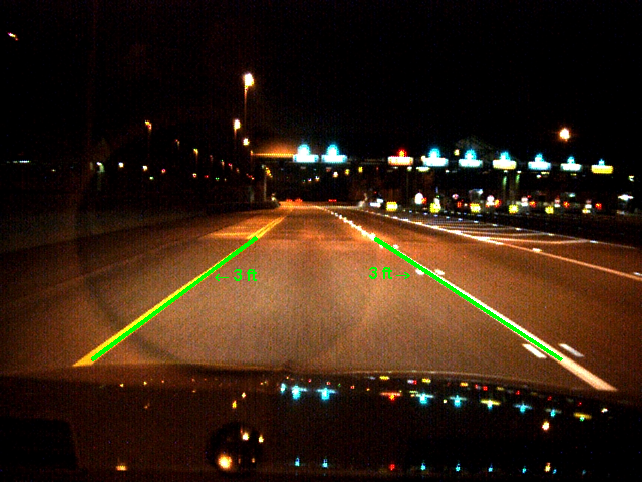
\includegraphics[width=0.237\textwidth]{IMG/res1.png}}\hspace{0.00001in}
  \subfloat[Presence of other markings on the road.]{\label{fig:temp_blur_after}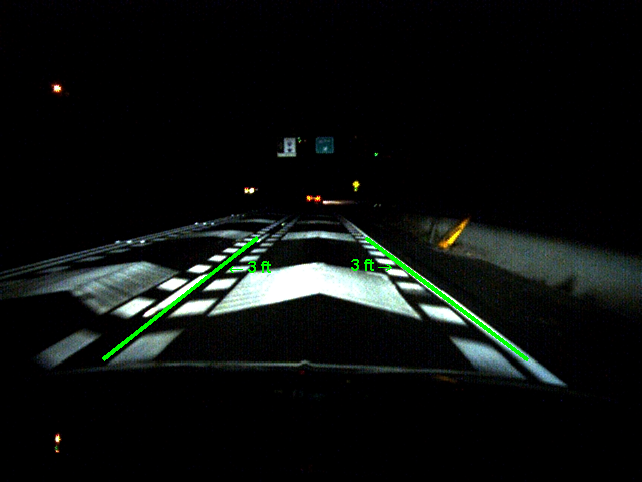
\includegraphics[width=0.237\textwidth]{IMG/res2.png}}\\
  \subfloat[Busy Highway.]{\label{fig:temp_blur_before}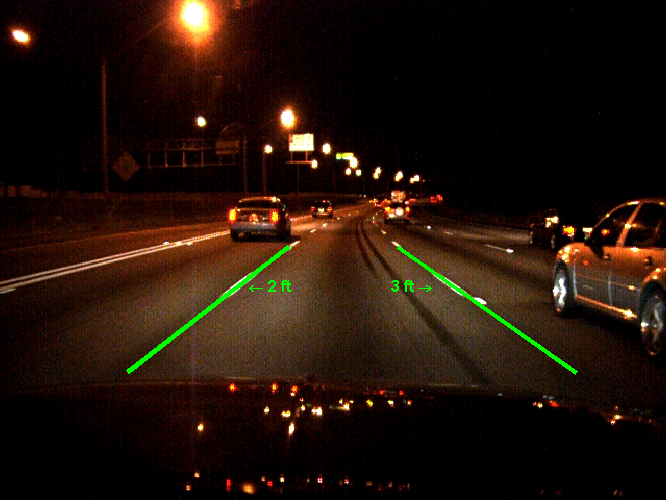
\includegraphics[width=0.237\textwidth]{IMG/res3.png}}\hspace{0.00001in}
  \subfloat[Busy city streets.]{\label{fig:temp_blur_after}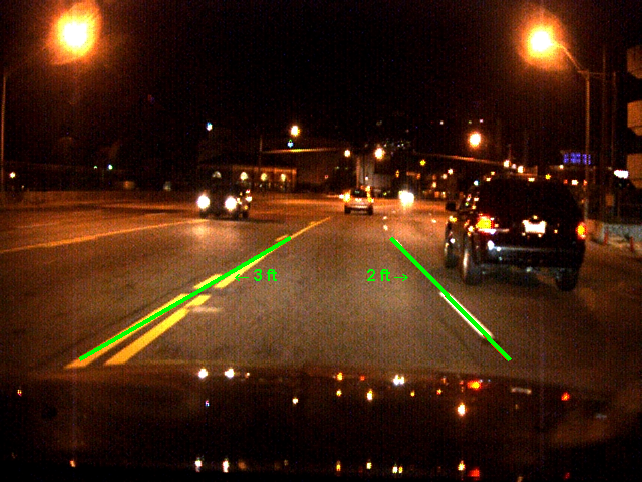
\includegraphics[width=0.237\textwidth]{IMG/res4.png}}\\
  \caption{Examples of accurate lane detection.}
  \label{fig:lane_detection}
\end{figure}
%As a result, computing the error between ground truth and prediction is not possible.
Defining a ground truth for the data is extremely tedious; hence, it is commonly avoided. Consequently, detections are generally quantified based on visual inspection.
\begin{figure}[htb!]
  \centering
  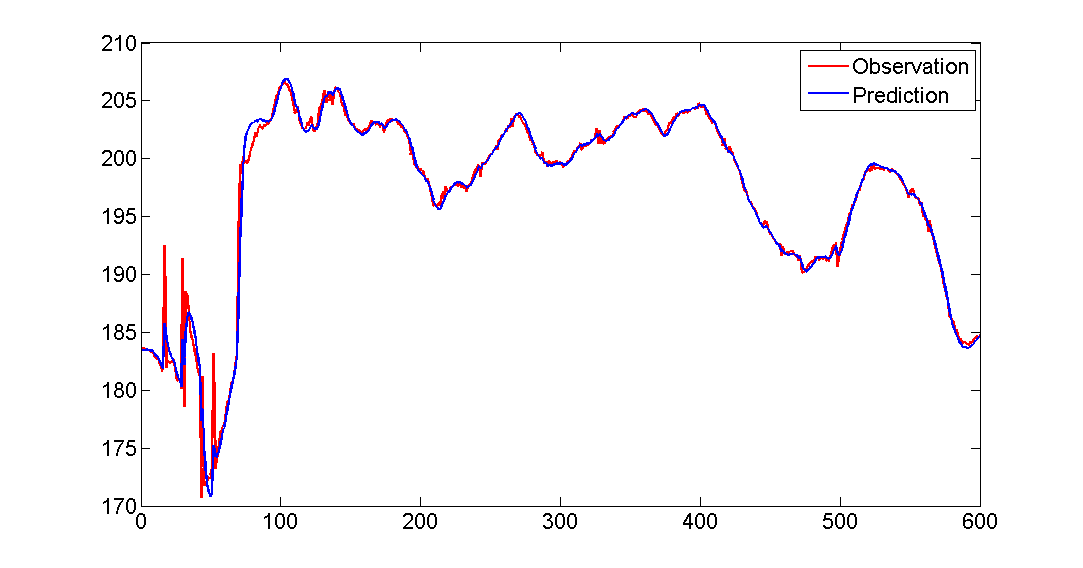
\includegraphics[width=0.5\textwidth]{IMG/obs_pred_rho.png}\\
  \caption{Comparison between observed and predicted values of $\rho$ over a range of frames. A blow up shows the Kalman filter smoothing the noisy measurements.}
  \label{fig:obs_pred_kalman}
\end{figure}
Despite noisy measurements, the Kalman filter recursively estimates the dynamics of the state vector. Fig. \ref{fig:obs_pred_kalman} shows a comparison between the observed and predicted value of $\rho$.
\begin{figure}[htb!]
  \centering
  \subfloat[Unsettled after a bump.]{\label{fig:lane_detection_wrong1}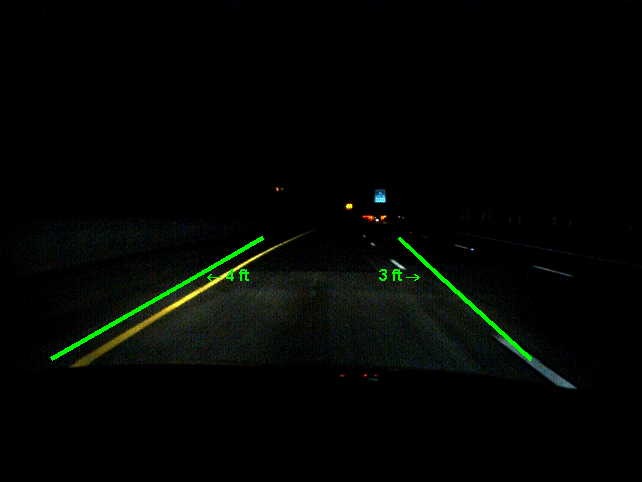
\includegraphics[width=0.237\textwidth]{IMG/fail1.png}}\hspace{0.00001in}
%  \subfloat[Lane change]{\label{fig:lane_detection_wrong2}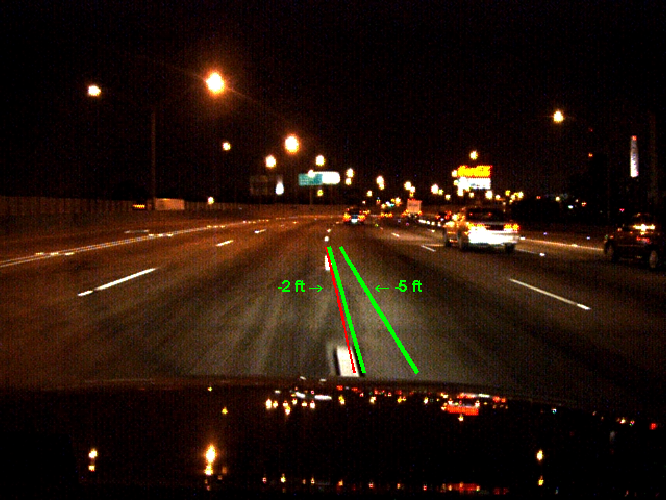
\includegraphics[width=0.237\textwidth]{IMG/fail2.png}}\\
  \subfloat[Poorly maintained city streets.]{\label{fig:lane_detection_wrong3}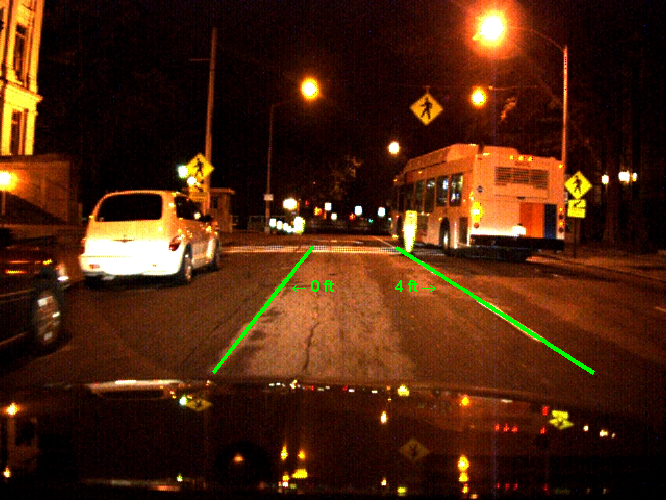
\includegraphics[width=0.237\textwidth]{IMG/fail3.png}}%\hspace{0.00001in}
%  \subfloat[Sharp turns]{\label{fig:lane_detection_wrong4}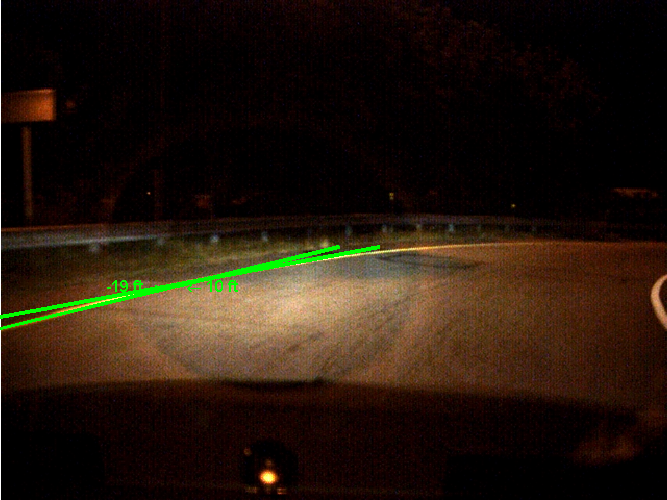
\includegraphics[width=0.237\textwidth]{IMG/fail4.png}}\\
  \caption{Examples of inaccurate lane detection.}
  \label{fig:lane_detection_wrong}
\end{figure}

A few instances of incorrect lane detections are also shown in Fig. \ref{fig:lane_detection_wrong}. Fortunately in Fig. \ref{fig:lane_detection_wrong1}, the Kalman filter is able to settle within a couple of milliseconds after passing the bump on the road. However, in Fig. \ref{fig:lane_detection_wrong3}, the absence of lane markers due to road aging and wear leads to the detection and tracking of false signals such as cracks.
\section{Conclusions}
\label{sec:concl}
The work presented in this paper is a significant improvement over the layered lane detection system presented in \cite{borkar_layered_2009}. The addition of features such as (1) Inverse Perspective Mapping (IPM), (2) Random Sample Consensus (RANSAC), and (3) Kalman filtering has added to the novelty and extension over the previous system. IPM aids in simplifying the process of finding candidate lane markers, while RANSAC helps in rejecting outliers within the estimations. Finally, the Kalman filter ignores minor perturbations and keeps the lane marker sequence on its track.

The data set used to test the accuracy of the proposed system was recorded on Interstate highways and city streets in and around Atlanta, GA. Despite the variety in traffic conditions and road quality encountered, the proposed system still yielded good performance as reflected in Table \ref{tab:laneDetectionCompare}.

\section{Future Work}
\label{sec:print}
Lane Departure Warning (LDW) will be implemented in the future. It will leverage from the lane detection system's ability to accurately determine the distance to the lane markers as shown in Fig. \ref{fig:lane_detection}. By analyzing the velocity and acceleration of lane marker movement, the driver can be notified of an up coming lane change. Further investigation is needed to enable day time lane detection. In addition, the implemented algorithms will be ported to C++ with the help of existing libraries like OpenCV and VXL to facilitate a real-time system.
%\vfill
%\pagebreak

% References should be produced using the bibtex program from suitable
% BiBTeX files (here: strings, refs, manuals). The IEEEbib.bst bibliography
% style file from IEEE produces unsorted bibliography list.
% -------------------------------------------------------------------------
\small
\bibliographystyle{IEEEbib}
\bibliography{refs}

\end{document}
